\chapter{A PX Model for \acp{PREG}}
\label{ch:model}
% A model that integrates constraints, aspects, instruments and methods, evaluators and game user researchers will benefit having a model that allows understanding dimensions (ayers and time) and elements that model PX in \acp{PREG}
There are several models to study \ac{PX} in digital games \autocite{Elson2014,Engl2013,Nackea2,Nacked,Fernandez2008,Mayra,DeKort2007b,Ferrara}. However, those models do not consider the physical rehabilitation constraints described in \autoref{ch:characterising} and the aspects, methods and instruments presented in \autoref{ch:aspects}. Consequently, those models are not adequate to study \acp{PREG}.

In this chapter, we propose a model for studying \ac{PX} in \acp{PREG}, which integrates existing research in \ac{PX} and the rehabilitation constraints that we identified previously. To design the model we employed the thematic content analysis to identify common constructs of \ac{PX} from eight existing models. We found that \ac{PX} should be studied considering two dimensions: time and level of abstraction. Then, we mapped the rehabilitation constraints from \autoref{ch:characterising} into those dimensions to propose a comprehensive \ac{PX} model for \acp{PREG}. Additionally, we propose a methodology that guides on the evaluation of \ac{PX} in \acp{PREG} using the model.

The remaining of this chapter is organised as follows: \autoref{sec:related_work_model} outlines the \ac{PX} models that we analysed to design our model. Then, \autoref{sec:model_design} presents the study that we conducted to design the model. After that, \autoref{sec:preg_px_model} describes the proposed model and its constructs. Moreover, \autoref{sec:methodology} the methodology to evaluate \acp{PREG} using the model. Finally, \autoref{sec:discussion_model} discusses the proposed model and \autoref{sec:conclusion_model} concludes the chapter.

% -----------------------------------------------
\section{Related work} % Related work %-----------------------------------------------
\label{sec:related_work_model}
The purpose of this study is to design a model to study \ac{PX} in \acp{PREG}. We have identified some constraints \autoref{ch:characterising} and aspects \autoref{ch:aspects} of \acp{PREG} from the field of physiotherapy. To design a comprehensive model we need to integrate those findings into current \ac{PX} models. Thus, this section presents the models that we considered to design our model.

We presented two models that we considered for our proposal in \autoref{sec:px_ux_models}. First, the \ac{IMP} model \autocite{Elson2014}, which describes \ac{PX} considering three elements, player, context and game. Also, the model suggests that \ac{PX} should be studied before, during and after interaction with a game occurs. Second, the Contextual Gameplay Experience Model \autocite{Engl2013}, which considers three elements similar to those of the \ac{IMP} model and is based on \autocite{Nackea2,Nacked}; i.e., game system, player and contextual influences. In this model, those elements are layers of abstraction, in which contextual influences is the most abstract layer and the game system is the most concrete one. It also suggests that \ac{PX} occurs before, during and after interaction occurs. Below, we present the other models that we use as a base to design our model.

\subsection{A PX Framework}
\textcite{Nackea2} present a \ac{PX} framework based on three layers of abstraction: the context, the player and the game system (See \autoref{fig:px_framework}). Context is the most abstract layer. It comprises the experience resulting from interacting with other players, games and technologies over a certain time. It involves the game community and its generated knowledge. The player layer represents the experience that influences and is influenced by the actions of players. The most concrete layer is the game system and comprises perceivable and technical experience generated by games.

The model presents interrelations among the layers. The context layer shapes players' perceptions of games, e.g., through a bad review. Meanwhile, the player the layer influences the context by generating knowledge about the game. Also, players provide content and data to shape game behaviour and adjust it to their preferences. Finally, the game system layer influences players' experience through its functionality and mechanics.

Finally, the model describes how each layer is affected by time. First, the game system layer is affected by technological changes. Second, the player layer evolves due to psychological and physiological changes. Finally, the context layer changes due to social, political or economic influences.

\begin{figure}[bth]
\myfloatalign
{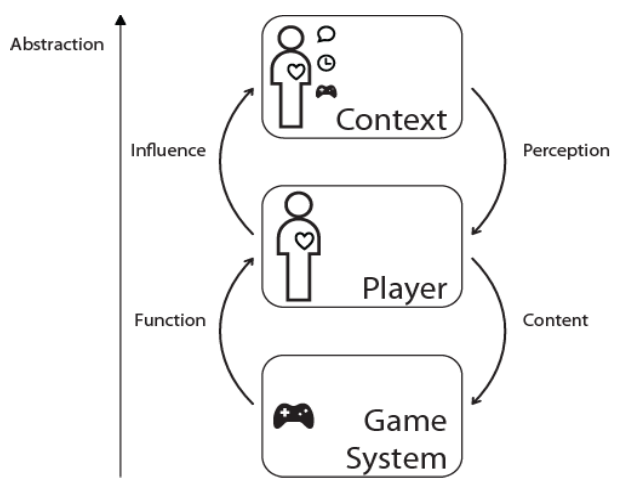
\includegraphics[width=.6\linewidth]{gfx/model/px_framework}} \quad
\caption[The PX Framework]{The \ac{PX} Framework \autocite{Nackea2}}\label{fig:px_framework}
\end{figure}

\subsection{The Game Usability Model}
\textcite{Nacked} presents the Game Usability Model that integrates \ac{PX} research into a single framework. It comprises nine entities that go from theoretical to practical and from concrete to abstract (See \autoref{fig:game_usa_model}). Three of those entities are theoretical constructs that affect \ac{PX}; i.e., technology, player and community. The technology entity is measured by the system quality and analysed using quality assurance. The player entity is measured by gameplay quality and studied using user experience analysis. Finally, the community construct is measured by the social quality and analysed using sociological studies.

This model intends to address three challenges that result when analysing \ac{PX}. The first challenge relates to \ac{PX} optimisation. According to the author, the interface of a game has to optimise \ac{PX} usability and functionality. The second challenge is the complexity of digital games, which are complex software programs due to content, controls, customisation and game design among others. The last challenge relates to time. \ac{PX} should be studied before, during and after interaction occurs. Before interaction, the state of the players and game marketing shape \ac{PX}. Also, the impact of an interaction on a player will affect preceding interactions.

\begin{figure}[bth]
\myfloatalign
{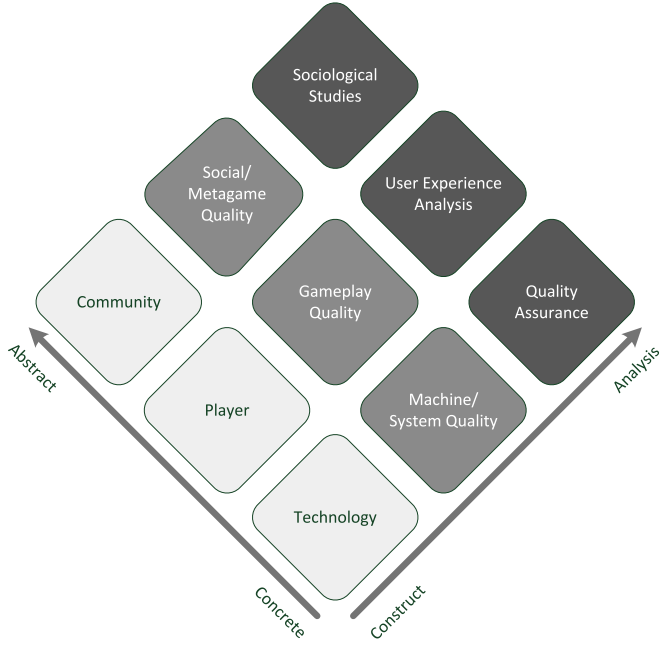
\includegraphics[width=.6\linewidth]{gfx/model/game_usa_model}} \quad
\caption[The Game Usability Model]{The Game Usability Model \autocite{Nacked}}\label{fig:game_usa_model}
\end{figure}

\subsection{The Game Experience Model}
\textcite{Fernandez2008} presents the Game Experience Model which suggests that the main result of game experience is fun. The model is based on three stages. First, the antecedents stage intends to capture the elements that motivate players to play a game, and lead to certain behaviours during an interaction. Second, the processing stage refers to the interaction moment between a player and a game. This stage depends on the players' motivation to play. Third, fun depends on the consequences of interacting with a game. These consequences can be cognitive such as thoughts and inferences, or emotional such as feelings.

The antecedents comprise players' demographics and game activity; i.e., previous experiences, game and hardware preferences and purpose. Those elements affect the motivation of players to start or continue playing a game.

Players' motivation determines the degree of attention and effort that they invest in a game during processing. According to the author, motivation also determines if players play using a serious or playful strategy. Additionally, games have pragmatic and hedonic attributes that affect \ac{PX}. Pragmatic attributes are assessed through the game interface and usability while hedonic attributes comprise the game mechanics (universe), the game features that trigger interactivity and the technology.

In \autocite{Fernandez}, the author conducted a study to prove the relations among the different elements of its model. The results showed that the years playing games and game genre preference define the user profile and purpose. Also, the author found that the user profile is related to motivation, but does not explain it. Furthermore, the results showed that when players are motivated, they can overcome usability shortcomings. Finally, the author found that high-quality technology and usability lead to universe appreciation.

\subsection{The Contextual Game Experience Model}
\textcite{Mayra} describes a model that considers the socio-cultural context of \ac{PX}. The author argues that games are played not only to experience fun, but also to facilitate social situations; e.g., when used to maintain or strengthen social relations. According to this model, the game experience is pre-defined, modified and post-defined by multiple dimensions. It relates to the immediate personal and social contexts. Thus, knowing players motivations, game habits and historical reasons to play is important to understand \ac{PX}. Additionally, the contexts for digital game production, the contexts provided by earlier forms for play (i.e., people's game literacy) and the context of social norms and values influence each other and shape game experience.

\subsection{People, Places and Play Research Framework}
\textcite{DeKort2007b} present a research framework that explores game experience as a situated experience formed by co-players, audience and spatial organisation. That is, the game experience is influenced by social contexts. The model is based on the evidence that people have better experiences when playing with or against players since social settings empower or diminish emotions. The social context of gaming comprises the presence of others, their ability to monitor and communicate with players, their role in the system (i.e., co-players or audience) and their relationships.

%-----------------------------------
\subsection{The Elements of \ac{PX}}
\textcite{Ferrara} presents a model to design and understand digital games. The model is divided into five planes, which have an associated short-term and long-term element. The planes should be addressed in the order presented below:

\begin{enumerate}
    \item \emph{Motivation}: it represents the players and their reasons to play a game. The short-term element is the \textit{players' interest} in the game, and the long-term elements are \textit{game rewards} that sustain interest over time.
    \item \emph{Meaningful choices}: it represents the mechanics that enable players to decide on the outcomes of game events. The short-term element is the players' \textit{strategy} and the long-term elements are the players' \textit{tactics}.
    \item \emph{Balance}: it refers to the appropriate level of challenge that players perceive as fair and equitable. The short and long-term elements are the game variables that enable balance.
    \item \emph{Usability}: it refers to the \ac{UX} and usability aspects of games. The short-term element of this plane is the players' sense of \textit{control}, and the long-term is the players' sense of \textit{mastery}.
    \item \emph{Aesthetics}: it refers to the aesthetic design of games. The short-term element is the players' \textit{sensory} perception of games (e.g., visual, haptic, audio), and the long-term element is the players' \textit{contemplative} perception of narrative.
\end{enumerate}

\section{Model design study} % Materials -----------------------------------
\label{sec:model_design}
\subsection{Aim of the study}
A study to propose a comprehensive model of \ac{PX} to evaluate \acp{PREG} is conducted. That is, to define a model that integrates current research in \ac{PX} and the characteristics and constraints of \acp{PREG} that we identified in \autoref{ch:characterising}.

\subsection{Procedure}
First, a literature review to identify existing \ac{PX} models is conducted. The models that serve to study \ac{PX}, game experience or gameplay experience are included. The eight documents presented in \autoref{sec:related_work_model}are selected. Four documents are identified in Scopus, and the remaining are extracted from their references. Then, the documents are reviewed and analysed to identify common \ac{PX} constructs a design a preliminary model. After that, the findings of the study that we presented in \autoref{ch:characterising} are mapped into the preliminary model to design the final one. An overview of the procedure is presented in \autoref{fig:modelDefiniton}.

\begin{figure}[bth]
\myfloatalign
{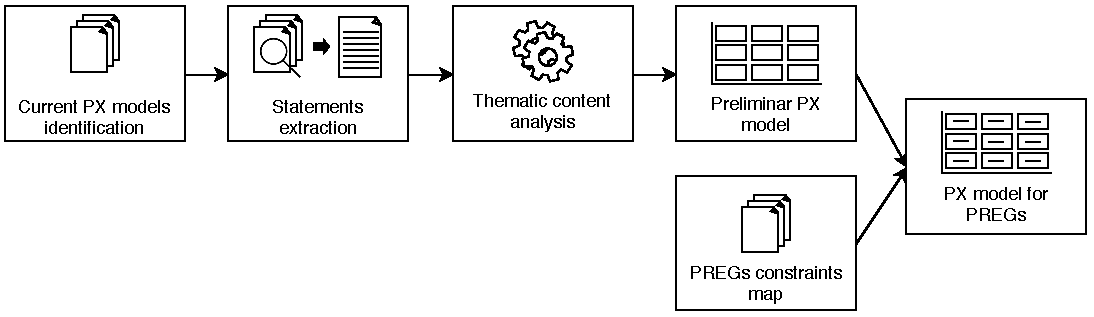
\includegraphics[width=\linewidth]{gfx/model/modelDefiniton}} \quad
\caption{Overview of model definition procedure}\label{fig:modelDefiniton}
\end{figure}

\subsubsection{Analysis}
The documents are analysed using the thematic analysis method \autocite{Braun}. The analysis is 'theory-driven' since we have identified a target data; i.e., \ac{PX} constructs and dimensions. The documents are reviewed to produce a list of relevant statements; i.e., those that are closely related to the aim of the study. Each statement was registered in a list including a reference to its source document. Then, preliminary codes are assigned to the statements. After that, the codes are iteratively grouped to identify potential themes, which are reviewed until defining the three final.

The thematic analysis of the reviewed documents\footnote{Existing PX models thematic analysis: \url{https://goo.gl/QvtG9G}} and the mapping of the \acp{PREG} constraints\footnote{PREGs constraints mapping into the PX model: \url{https://goo.gl/wdn57M}} are available online.

%-----------------------------------
\section{PX Model for PREGs} % Findings -----------------------------------
\label{sec:preg_px_model}
After conducting the thematic analysis, 104 initial codes were identified and iteratively grouped until we achieved a total of three main themes. The first theme is \textit{layers of abstraction} which represent the main actors that may influence \ac{PX}. The second theme is \textit{moments of \ac{PX}}, which represents the moments in which \ac{PX} should be studied. The last theme refers to the relations among the first two themes.

\subsubsection{Layers of abstraction}
\label{sec:layers_abstraction}
The layers of abstraction represent the actors that influence \ac{PX} \autocite{Nacked,Nackea2,Engl2013,Elson2014}. In this study, we identified three main layers of abstraction; i.e., \textit{the context, the player} and \textit{the game system}. \ac{PX} should be studied in a situational perspective \autocite{Nacked,DeKort2007b} since it influences players' perceptions \autocite{Elson2014} behaviours and interactions \autocite{Engl2013,DeKort2007b}. \ac{PX} represents the individual experience of playing a game \autocite{Engl2013,Nackea2}, that is, every experience is shaped by the unique perspective \autocite{Fernandez2008} and properties \autocite{Nacked} of each player. Lastly, games are designed to offer pleasurable experiences to players, although these are complex pieces of software \autocite{Nackea}, and may have numerous interaction possibilities, challenges and complex controls \autocite{Nacked} that alter \ac{PX}.

Although \textcite{Nackea2} proposed a set of relations among the three layers of abstraction,which we described previously; we identified new relations regarding the use of \acp{PREG} in physical therapy. In that case, the game system assists physical therapy, and physiotherapists shape \ac{PX} by configuring the game system and supervising players. The layers of abstraction and their relations are illustrated in \autoref{fig:layersOfAbstraction}.

\begin{figure}[bth]
\myfloatalign
{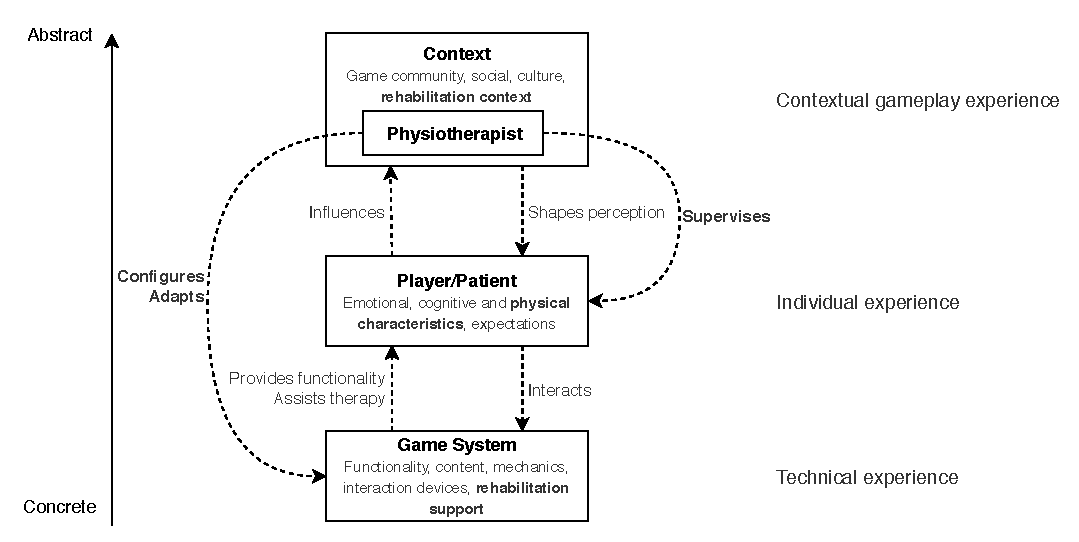
\includegraphics[width=\linewidth]{gfx/model/layersOfAbstraction}} \quad
\caption{\ac{PX} layers of abstraction and relations among them} \label{fig:layersOfAbstraction}
\end{figure}

\subsubsection*{Context}

The \textit{Context} is the most abstract layer and forms the contextual gameplay experience and may empower player's positive emotions and enhance or diminish their negative ones \autocite{DeKort2007b}. It shapes the experience of players through environmental influences that affect players' motivation to play a game \autocite{Elson2014}. Studying the context layer in the long-term may imply conducting sociological studies \autocite{Nacked}.

The social context of playing games \autocite{Mayra,DeKort2007b,Elson2014} comprises the influence of other people. First, co-players presence \autocite{Nacked,Nackea2,Nackea,DeKort2007b,Elson2014,Mayra} (i.e., co-located, mediated, simulated or absent) may enhance \ac{PX} depending on players preferences \autocite{DeKort2007b}. Similarly, the presence of an audience; i.e., people that monitors players' actions and emotions, may influence \ac{PX} \autocite{DeKort2007b,Mayra,Nackea2}. In the case of \acp{PREG}, physiotherapists represent a permanent audience that should be studied when evaluating \ac{PX}. 

Furthermore, game communities \autocite{Nacked,Nackea2,Elson2014} shape the social quality of games; these enable players to interact with others using different forms of communication \autocite{Elson2014}, and offer opportunities for review and discussion \autocite{Nacked}. Consequently, game communities influence players perception of certain games or games genres \autocite{Nackea,Nackea2}. Likewise, the game market \autocite{Elson2014,Nackea} influences players preferences and choice.

When playing a game, the location \autocite{Engl2013,Elson2014}, spatial organisation \autocite{DeKort2007b} and technical infrastructure \autocite{Elson2014} may enhance or diminish the experience. This is relevant for \acp{PREG} sine these employ interaction devices such the Kinect, thereby requiring enough space to locate players at an adequate distance.

Moreover, cultural parameters such as values and norms \autocite{Elson2014,Mayra} may allow or prevent playing a game.

The rehabilitation context constraints presented in \autoref{sec:reh_context_constraints} may extend this layer. These constraints include institutions norms and regulations, physiotherapists' participation, the use of assisting objects and therapy related activities.

The context layer changes based on sociological, economic or political changes that affect players \autocite{Nackea2}.

\subsubsection*{Player/Patient}

The \textit{Player} layer represents the individual experience of a person when playing a game. This layer comprises the characteristics of s player as individual \autocite{Elson2014} such as his/her cultural \autocite{Elson2014} and historical \autocite{Mayra} background, demographic data (e.g, age, gender, literacy) \autocite{Elson2014,Fernandez2008,Ferrara} and personal traits \autocite{Elson2014}. Analysing players' characteristics is important to offer a compelling experience since each kind of player may have different expectations. For instance, playful oriented players are curious, explorers and focused on the present, whereas the serious oriented players are goal oriented and focus efforts on the future \autocite{Fernandez2008}.

Also, this layer involves factors related to previous gaming experiences of a player including memories \autocite{Elson2014}, game activity (e.g. games and hardware preferences/aversions, time playing and frequency) \autocite{Fernandez2008,Nackea2,Nacked,Mayra} and games literacy \autocite{Mayra}.

In addition to entertainment, a player may start playing a game with other purposes such as socialising, training and rehabilitating. Accordingly, the player layer comprises the motivations and expectations of a player that are not related to the game itself; these include the need for interaction, relatedness or affiliation \autocite{DeKort2007b,Mayra}, and the need to rehabilitate using \acp{PREG}.

Furthermore, this layer includes the processes and responses that players experience during and after playing a game. The processes and responses can be emotional such as fun, motivation, pleasure, engagement, \autocite{Fernandez2008,Ferrara} and enjoyment \autocite{Nacked}; cognitive such as mastery, control \autocite{Ferrara}, attention, thoughts and opinions \autocite{Fernandez2008}; and physical such as \c{HR}, motion range and balance.

In the case of \acp{PREG}, the physical processes and responses are relevant since players are recovering from a physical impairment. Moreover, the player layer comprises the patients' related constraints presented in \autoref{sec:reh_patients_constraints}.

The player/patient layer changes gradually over time based on psychological and physiological processes experienced by players \autocite{Nackea2}.

\subsubsection*{Game System}
The \textit{Game System} is the most concrete layer and represents the perceivable and technical experience elicited when playing a game \autocite{Nackea2,Elson2014,Nackea,Nacked}. This layer depends on technological limits or advances to evolve \autocite{Fernandez2008}. Studying the game system in \ac{PX} is important since a game is a complex software system \autocite{Mayra,Nackea} and its design impacts directly on the experience that a player may have.

This layer comprises general prerequisites to ensure the availability of a game; this includes attraction factors \autocite{Elson2014}, \ac{QA} \autocite{Nacked} and the learning curve, which should meet players skills to avoid frustration \autocite{Nacked}. The general prerequisites may involve technical \autocite{Fernandez2008,Engl2013,Nackea2} and marketing \autocite{Nacked} issues.

Furthermore, the game system layer includes interactive characteristics such as game design \autocite{Nacked}, content \autocite{Elson2014,Nackea2,Fernandez2008}, mechanics \autocite{Elson2014,Ferrara}, rules \autocite{Nackea}, universe (i.e., plot, characters and realism) \autocite{Fernandez2008,Ferrara}, interface, media \autocite{DeKort2007b,Fernandez2008}, aesthetics \autocite{Ferrara}, playability \autocite{Engl2013,Fernandez2008} and interactivity (i.e., game challenge, pace and responsiveness) \autocite{Fernandez2008}. Additionally, this layer involves the game technology \autocite{Engl2013,Fernandez2008}; i.e., the interaction devices.

The game system comprises the components that assist a rehabilitation therapy. It involves the interaction devices constraints presented in \autoref{sec:interation_dev_constraints}. And the constraints presented in \autoref{sec:reh_goal_constraints} that impose prerequisites on the game system such as patients' safety assurance, feedback provision about progress and exercise correctness, movement mapping correctness and gameplay time.

The game system layer changes over time according to technological steps, which are mainly imposed by consoles manufacturers \autocite{Nackea,Nackea2}.

\subsubsection{Moments of \ac{PX}}
We identified that \ac{PX} is a comprehensive phenomenon that occurs not only during the actual gameplay \autocite{Mayra}; thus, it should be studied along three moments \autocite{Elson2014,Fernandez2008,Nackea2,Nackea,Nacked} (i.e., before, during and after playing a game). \textcite{Elson2014} name these three moments pre-game, game and post-game effects; whereas \textcite{Fernandez2008} names them antecedents, processing and consequences. Moreover, \textcite{Mayra} claims that \ac{PX} is pre-defined, modified and post-defined by multiple dimensions. We name these moments as \textit{antecedents, interaction} and \textit{effects} since those represent what each moment refers to. The moments of \ac{PX} and their relation are illustrated in \autoref{fig:temporalDimension}.

\begin{figure}[bth]
\myfloatalign
{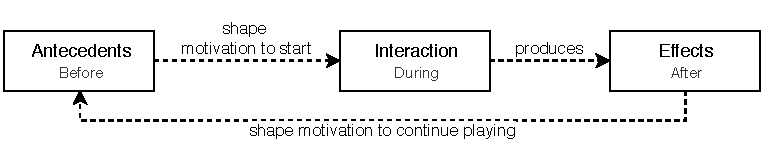
\includegraphics[width=.9\linewidth]{gfx/model/temporalDimension}} \quad
\caption{Moments of \ac{PX}}\label{fig:temporalDimension}
\end{figure}

\subsubsection*{Antecedents}
The antecedents are everything that occurs before the actual gameplay and shape players' motivation to start playing a game \autocite{Fernandez2008,Ferrara}. In the case of \acp{PREG}, the antecedents shape physiotherapists' motivation to use a game in physical therapy.

\subsubsection*{Interaction}
The interaction depends on the antecedents and occurs when players play a digital game \autocite{Elson2014,Fernandez2008,Nacked}. This moment shapes the players' perception of a game depending on their experience \autocite{Fernandez2008}. In \acp{PREG}, the interaction moment would also affect physiotherapists' perception. The effects of interaction have a direct impact on future experiences.

\subsubsection*{Effects}
The effects are positive or negative consequences that result from the interaction moment \autocite{Fernandez2008}; these form a feedback loop that affects future interactions \autocite{Nacked,Elson2014} shaping players' motivation to continue playing a game. The effects can be short-term and long-term. Short-term effects are temporary changes in thoughts, feelings and behaviours right after an interaction. Whereas, long-term effects are consequences of repeated episodes of interaction \autocite{Elson2014}.

\subsubsection{Layers of abstraction over the moments of \ac{PX}}
\label{sec:rel_among_dimensions}
The layers of abstraction can be studied throughout the moments of \ac{PX}. We mapped the layers' components that we present previously (See \autoref{sec:layers_abstraction}) into these moments as illustrated in \autoref{fig:pxModel} and described below.

\begin{figure}[bth]
\myfloatalign
{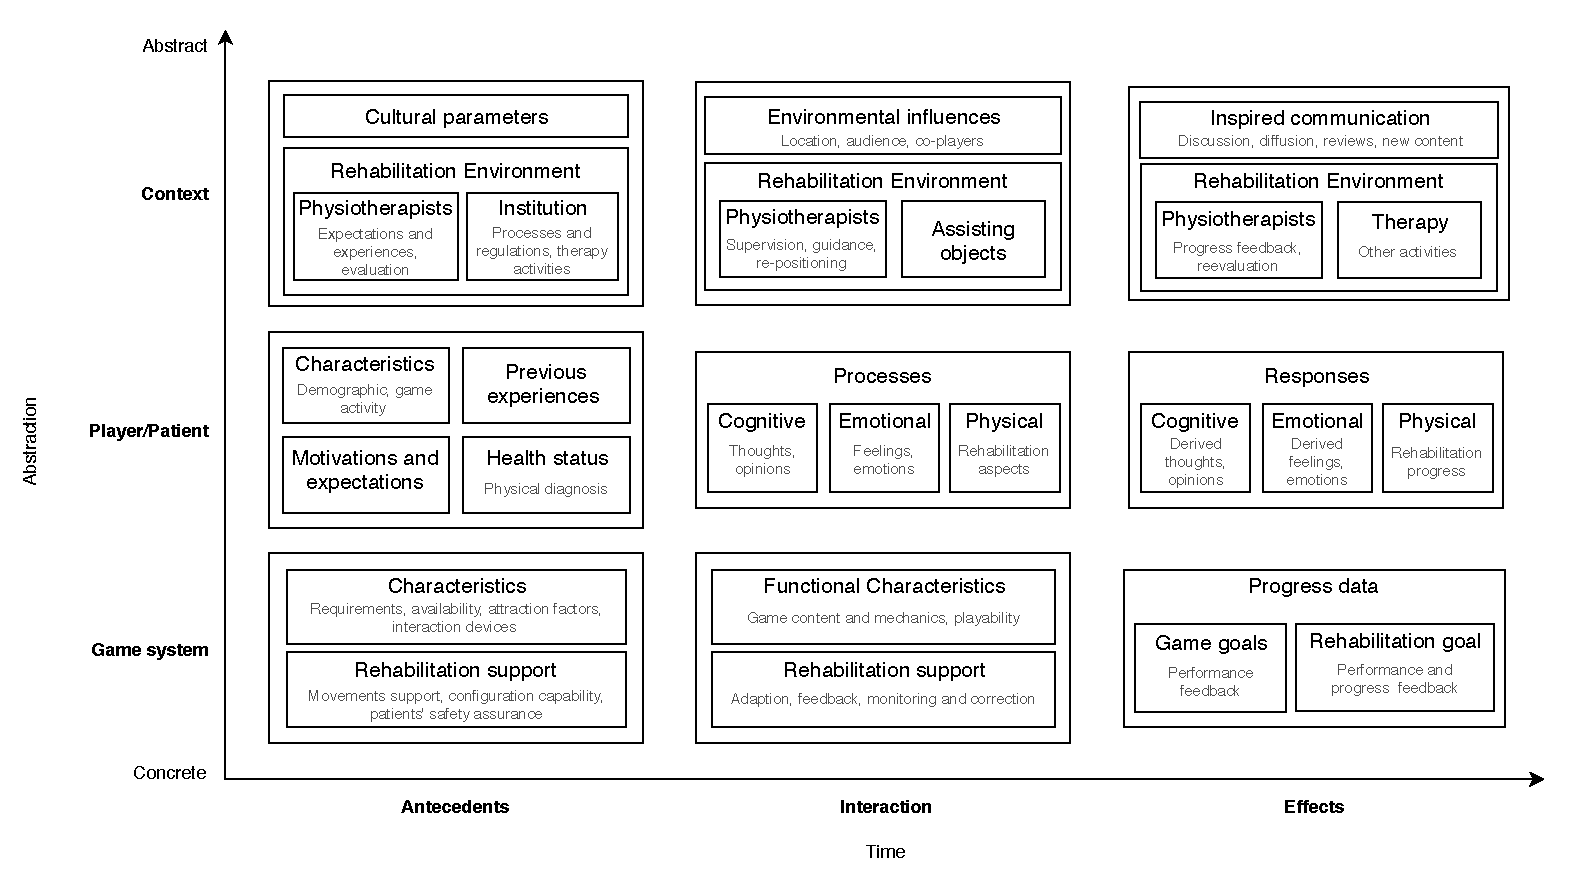
\includegraphics[width=\linewidth]{gfx/model/pxModel}} \quad
\caption{\ac{PX} Layers of Abstraction over Time}\label{fig:pxModel}
\end{figure}

\subsubsection*{Layers of abstraction during the antecedents}
During the antecedents, the \textit{context} comprises the elements affect players' opportunity of playing a game. That includes cultural parameters, the game community, the health institution regulations and physiotherapists' expectations, criteria and experience with \acp{PREG}.

The \textit{player/patient} layer is defined by player's characteristics, game experience, motivations and expectations (including those regarding their physical therapy and the use of \acp{PREG}) and health status (i.e., impairment, physical skills, functional independence). 

On the other hand, the \textit{game system} layer comprises general prerequisites of games such as \ac{QA} and attraction factors. In physical rehabilitation, it comprises the capability of the game to assist treatments.

\subsubsection*{Layers of abstraction during the interaction}
During the interaction, the \textit{context} layer includes influences from the environment and the rehabilitation process (e.g. physiotherapists participation and use of assisting object). The \textit{player/patient} layer comprises the sum of cognitive, emotional and physical processes and behaviours experienced by players while playing a game. Lastly, the \textit{game system} layer comprises the characteristics that enable interaction and rehabilitation (adaptation, feedback provision, monitoring, exercise correction and physical objects support).

\subsubsection*{Layers of abstraction during the effects}
The effects of the \textit{context} layer include all forms of communication caused or inspired by playing a game, including the physiotherapists' feedback and re-evaluation and other therapy related tasks such as paper-work. The \textit{player/patient} layer effects comprise cognitive, emotional and physical responses derived from an interaction episode. The physical responses are associated with the expected rehabilitation goal. The \textit{game system} layer comprises the quality of progress data regarding game and rehabilitation goals.

% -----------------------------------------------
\section{A Methodology to Evaluate PX in PREGs}
\label{sec:methodology}
Evaluating \ac{PX} in \acp{PREG} requires using a methodology that matches the model that we presented in the previous section. An evaluation may cover one or more moments and layers of abstraction of \ac{PX}. Also, the aspects to be assessed depend on the moments and layers being evaluated. Evaluators should select the adequate methods and instruments to evaluate those aspects properly. Lastly, such methodology may enable iterative evaluations since \ac{PX} evolves after each interaction of a player with a game. For instance, to evaluate the impact of a \ac{PREG} on a patient's rehabilitation process, an evaluator should assess the \textit{player/patient} layer throughout the three moments of \ac{PX}, during a whole treatment. The evaluator should identify relevant aspects to evaluate such as range of motion, which can be assessed using goniometry. Those aspects may be measured before, during and after several interaction episodes.

In this section, we present a methodology that attempts to guide evaluators in the process of selecting evaluation aspects, methods and instruments to assess \ac{PX} in \acp{PREG}. This methodology is intended to be used along the whole development life cycle. It can be used iteratively to refine the outcomes of each stage after each evaluation. The stages of our methodology are illustrated in \autoref{fig:PXEvaluationMethodology} and detailed below.

\begin{figure}[bth]
\myfloatalign
{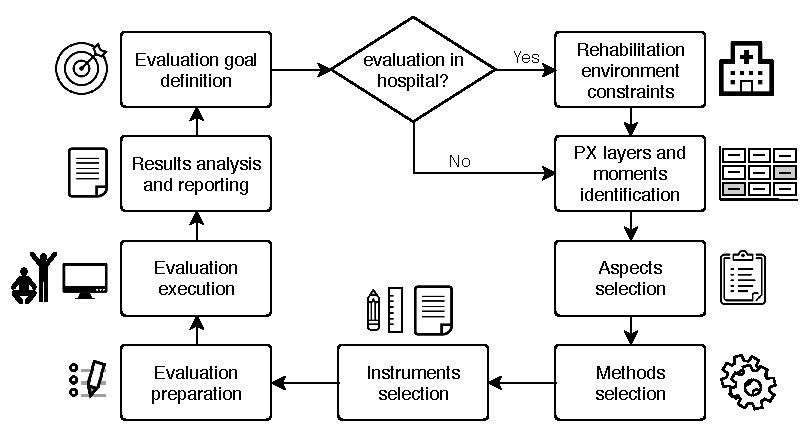
\includegraphics[width=\linewidth]{gfx/model/PXEvaluationMethodology}} \quad
\caption{Stages of the proposed methodology}\label{fig:PXEvaluationMethodology}
\end{figure}

\subsection{Evaluation goal definition}
Evaluators should now define the evaluation goal based on the development maturity of the \ac{PREG}. First, evaluators should focus on assuring patient’s safety. First, they should concentrate on the evaluating the antecedents of \ac{PX}; and then they can start assessing the interaction and effects moments of \ac{PX}.

\subsection{Rehabilitation environment constraints}
If required, evaluators should identify constraints additional to those presented in \autoref{ch:characterising}; these include constraints imposed by regulations and internal processes of the health institution where evaluation may occur. They should concentrate on the logistics that are required to perform an evaluation including participants, location, regulations, among others. When a \ac{PREG} consists of collection of mini-games, each mini-game should be evaluated separately.

\subsection{\ac{PX} layers and moments identification}
Evaluators identify which layers of abstraction and moments of \ac{PX} should be evaluated to achieve the evaluation goal established in the previous stage.

\subsection{Evaluation aspects selection}
Selecting the aspects to be evaluated is a crucial task to be overcome when preparing an evaluation. This selection depends on the layers and moments of \ac{PX} to be evaluated, the available resources and the development maturity of the evaluated \ac{PREG}. A discussion about relevant aspects to be evaluated in \acp{PREG} was presented in \autoref{sec:rehab_aspects}. \autoref{tab:aspectsModelMappingContext}, \autoref{tab:aspectsModelMappingPlayer} and \autoref{tab:aspectsModelMappingGame} present a mapping between those aspects and each moment of \ac{PX} for the context, the player/patient and the game system layers of abstraction respectively. A mapping that includes a larger set of aspects is available online\footnote{Mapping of evaluation aspects into the PX Model: \url{https://goo.gl/K4rked}}

\begin{table}[h]
\caption{Aspects to evaluate the context layer over time}
\label{tab:aspectsModelMappingContext}
\myfloatalign
\resizebox{0.9\linewidth}{!}{
\begin{tabular}{p{7cm}llp{2cm}}
\toprule
\multirow{2}{*}{\spacedlowsmallcaps{Aspect(s)}} & \multicolumn{3}{c}{\spacedlowsmallcaps{Moment of PX}} \\
\cline{2-4}
 & \spacedlowsmallcaps{Antecedents} & \spacedlowsmallcaps{Interaction} & \spacedlowsmallcaps{Effects} \\
\midrule
Physiotherapists preference, expectations & X &  &  \\
\midrule
Game diffusion & X &  & X \\
\midrule
Location & X & X &  \\
\midrule
Competence, collaboration &  & X &  \\
\midrule
Game knowledge generation &  &  & X \\
\midrule
Institutions regulations/processes & X &  &\\
\midrule
\bottomrule
\end{tabular}}
\end{table}

\begin{table}[h]
\caption{Aspects to evaluate the player/patient layer over time}
\label{tab:aspectsModelMappingPlayer}
\myfloatalign
\resizebox{\linewidth}{!}{
\begin{tabular}{p{10cm}llp{2cm}}
\toprule
\multirow{2}{*}{\spacedlowsmallcaps{Aspect(s)}} & \multicolumn{3}{c}{\spacedlowsmallcaps{Moment of PX}} \\
\cline{2-4}
 & \spacedlowsmallcaps{Antecedents} & \spacedlowsmallcaps{Interaction} & \spacedlowsmallcaps{Effects} \\
\midrule
Emotion & X & X & X \\ \midrule
Negative-positive affect &  & X & X \\ \midrule
Interest & X & X & X \\ \midrule
Story & X & X &  \\ \midrule
Accomplishment &  & X & X \\ \midrule
Engagement, challenge, flow, enjoyment, fun, immersion, absorption, presence, attention, tension, curiosity &  & X &  \\ \midrule
Clarity of game goals, ease of use, cognitive load, learnability &  & X &  \\ \midrule
Preference & X &  & X \\ \midrule
Rehabilitation goal achievement &  &  & X \\ \midrule
Physical rehabilitation aspects & X & X* & X \\ \midrule
Movement meaningfulness &  & X &  \\ \midrule
Tutorial understanding &  & X &  \\
\midrule
\bottomrule
\end{tabular}}
\\ * If supported by the \ac{PREG} or other equipment
\end{table}

\begin{table}[htb]
\caption{Aspects to evaluate the game system layer over time}
\label{tab:aspectsModelMappingGame}
\myfloatalign
\resizebox{0.9\linewidth}{!}{
\begin{tabular}{p{7cm}llp{2cm}}
\toprule
\multirow{2}{*}{\spacedlowsmallcaps{Aspect(s)}} & \multicolumn{3}{c}{\spacedlowsmallcaps{Moment of PX}} \\
\cline{2-4}
 & \spacedlowsmallcaps{Antecedents} & \spacedlowsmallcaps{Interaction} & \spacedlowsmallcaps{Effects} \\
\midrule
Playability & X & X & X \\ \midrule
Configuration capability & X &  &  \\ \midrule
Adaptation capability &  & X &  \\ \midrule
Movement mapping correctness & X &  &  \\ \midrule
Movement mapping completeness & X &  &  \\ \midrule
Monitoring, movement correction, movement correctness feedback &  & X & \\ \midrule
Progress feedback &  & X & X \\ \midrule
Tutorial completeness & X &  &  \\ \midrule
Functionality, aesthetics, point of view &  & X &  \\ \midrule
\bottomrule
\end{tabular}}
\end{table}

\subsection{Evaluation methods selection}
Evaluators should select methods based on the selected aspects and available re-sources; e.g., experts, participants, location and evaluation instruments. A discussion about relevant methods to evaluate in \acp{PREG} was presented in \autoref{sec:rehab_methods}. Moreover, \autoref{tab:methodsModelMappingContext}, \autoref{tab:methodsModelMappingPlayer} and \autoref{tab:methodsModelMappingGame} present the methods that evaluators can use to assess the context, the player/patient and the game system layers of abstraction respectively, during each moment of \ac{PX}.

\begin{table}[htb]
\caption{Evaluation methods for the context layer over time}
\label{tab:methodsModelMappingContext}
\myfloatalign
\resizebox{0.8\linewidth}{!}{
\begin{tabular}{p{6cm}llp{2cm}}
\toprule
\multirow{2}{*}{\spacedlowsmallcaps{Method}} & \multicolumn{3}{c}{\spacedlowsmallcaps{Moment of PX}} \\
\cline{2-4}
 & \spacedlowsmallcaps{Antecedents} & \spacedlowsmallcaps{Interaction} & \spacedlowsmallcaps{Effects} \\
\midrule
Questionnaires & X & X & X \\ \midrule
Interview & X &  & X \\ \midrule
Field-Behavioural observation & X & X &  \\ \midrule
Focus groups & X &  & X \\ \midrule
Co-discovery learning &  & X &  \\ \midrule
Peer tutoring &  & X &  \\ \midrule
Prisoner dilemma task &  & X &  \\ \midrule
Ethnography & X & X & X \\ \midrule
Cultural debugging & X &  &  \\ \midrule
Multiplayer game metrics &  & X &  \\ \midrule
\bottomrule
\end{tabular}}
\end{table}

\begin{table}[h]
\caption{Evaluation methods for the player/patient layer over time}
\label{tab:methodsModelMappingPlayer}
\myfloatalign
\resizebox{0.8\linewidth}{!}{
\begin{tabular}{p{6cm}llp{2cm}}
\toprule
\multirow{2}{*}{\spacedlowsmallcaps{Method}} & \multicolumn{3}{c}{\spacedlowsmallcaps{Moment of PX}} \\
\cline{2-4}
 & \spacedlowsmallcaps{Antecedents} & \spacedlowsmallcaps{Interaction} & \spacedlowsmallcaps{Effects} \\
\midrule
Questionnaires & X & X & X \\ \midrule
Interview & X &  & X \\ \midrule
Video recording &  & X &  \\ \midrule
Field-Behavioural observation & X & X & X \\ \midrule
Think-aloud protocol &  & X &  \\ \midrule
Focus groups & X & X & X \\ \midrule
Question-asking protocol &  & X &  \\ \midrule
Biometrics analyse & X &  & X \\ \midrule
\ac{EEG}, \ac{EMG}, \ac{EDA}, \ac{HR} & X & X & X \\ \midrule
Body movement coding &  & X &  \\ \midrule
Eye-tracking &  & X &  \\ \midrule
Persona modelling & X &  &  \\ \midrule
Player modelling & X &  &  \\ \midrule
Physical rehabilitation tests & X &  & X \\ \midrule
Physiotherapist observation & X & X & X \\ \midrule
\bottomrule
\end{tabular}}
\end{table}


\begin{table}[htb]
\caption{Evaluation methods for the game system layer over time}
\label{tab:methodsModelMappingGame}
\myfloatalign
\resizebox{0.8\linewidth}{!}{
\begin{tabular}{p{6cm}llp{2cm}}
\toprule
\multirow{2}{*}{\spacedlowsmallcaps{Method}} & \multicolumn{3}{c}{\spacedlowsmallcaps{Moment of PX}} \\
\cline{2-4}
 & \spacedlowsmallcaps{Antecedents} & \spacedlowsmallcaps{Interaction} & \spacedlowsmallcaps{Effects} \\
\midrule
\ac{QA} & X & & \\ \midrule
\ac{RITE} & X & X &  \\ \midrule
Heuristic evaluation & X & X & X \\ \midrule
Guidelines or standard inspections & X & X & X \\ \midrule
Cognitive walkthrough & X & X & X \\ \midrule
Pluralistic walkthrough & X & X & X \\ \midrule
Gameplay metrics &  & X &  \\ \midrule
Game logs &  & X &  \\ \midrule
A/B Testing & X & X & X \\ \midrule
\bottomrule
\end{tabular}}
\end{table}

\subsection{Evaluation instruments selection}
Evaluators should select evaluation instruments based on the aspects and methods involved in the evaluation. Evaluation instruments for \acp{PREG} may be borrowed from \ac{GUR}, \ac{UX} and physical rehabilitation fields. A discussion about relevant instruments to evaluate in \acp{PREG} was presented in \autoref{sec:rehab_instruments}. Additionally, a mapping between evaluation aspects and instruments is available online\footnote{Mapping between evaluation aspects and instruments: \url{https://goo.gl/j9suDc}}

\subsection{Evaluation preparation}
Evaluators should prepare all logistics associated to evaluation and a test protocol based on the outcomes of the previous stages.

\subsection{Evaluation execution}
Evaluators conduct the planned evaluation. The evaluation may occur in a laboratory or at a health institution.

\subsection{Results analysis and reporting}
Evaluators analyse the data collected during evaluation and reports the findings and recommendations considering the evaluation goal. This is a common task on usability and \ac{UX} evaluation; thus, similar approaches can be employed.


\section{Discussion} % Discussion %-----------------------------------------------
\label{sec:discussion_model}
%%%%% Reiterate the Research Problem/State the Major Findings:
% Comprehensive model for \acp{PREG}
% PX studied in two dimensions: time: before, during, after; level of abstraction: context, player/patient, game system + constraints identified in previous study
% Integrate models to explain relations among layers and dimensions of \a{PX}
Although there are models to study \ac{PX}, these are designed based on entertainment games and do not integrate the constraints imposed by the use of \acp{PREG} in physical therapy. Consequently, we conducted a qualitative study to explore the constructs and concepts of existing \ac{PX} models and integrate them with the rehabilitation constraints that we identified in a previous study (See \autoref{ch:characterising}). The purpose of the study was to design a comprehensive model to study and understand \ac{PX} in \acp{PREG}. The model comprises two dimensions, i.e., time and abstraction. Additionally, we proposed a methodology that guides \ac{PX} evaluators on the evaluation of \ac{PX} covering the model dimensions.

%%%%%%% Explain the Meaning of the Findings and Why They are Important: expected? unexpected? (explain these especially). unusual or unanticipated patterns or trends that emerged from your results and explain their meaning in relation to the research problem.
% PX study as an iterative process, consequences affect -> future antecedents
Regarding time, \ac{PX} comprises three moments: the interaction episode (during), its antecedents (before), and its effects (after). The antecedents shape players' motivation to start playing, and the effects shape players' motivation to continue playing. As a consequence, studying or evaluating \ac{PX} requires an iterative process since the effects of a gameplay episode become the antecedents of future interactions.

We identify three layers of abstraction in the literature, the context, the player (renamed as player/patient) and the game system. To propose a model to evaluate \acp{PREG}, we map the constraints that we identified in \autoref{ch:characterising} into each layer. The context was extended with the rehabilitation environment constraints imposed by the health institutions, the physiotherapists' participation and therapy related activities. The player layer was enriched with those constraints that identify players as patients of physical therapy. The game system was extended with those constraints that indicate requirements that \acp{PERG} should meet to be used in physical therapy.

% Expected: important role of physios adn insitutions as antecedents to trigger interaction, physios as partipators of interaction and progress feedback (/)
% consider physiotherapists vision (clinical(evaluators) and as users)
Our findings highlight the role of the rehabilitation environment at each moment of \ac{PX} in the context layer. We highlighted the role of physiotherapists and institutions as antecedents that may cause or prevent the use of \acp{PREG} with a patient. To study that, one should consider health institutions regulations and the physiotherapists' expectations, previous experiences and role as responsible for patients. Also, the rehabilitation context may affect interaction episodes since physiotherapists' should guide and supervise patients while playing. Finally, the effects produced by the rehabilitation context include physiotherapists' feedback provision reevaluation and additional therapy activities required by institutions.

%Understand the role of the Game system in the therapy. And the rehab env. in the game
Regarding the game system layer of abstraction, the model defines the characteristics on which evaluations should focus. Additional to the characteristics of entertainment games, we could identify that assisting a rehabilitation goal, supporting a set of physical movements and assuring patients' safety are relevant antecedents to use a game with physical therapy patients. Also,  the capability of a \ac{PREG} to enable or facilitate adaptation to patients' needs, provide relevant feedback, and monitor patients should be assessed during the interaction episodes. Whether it should facilitate or enable those tasks depends on its degree of autonomy. After an interaction episode, the quality of feedback about patients' game and physical progress should be assessed.

% Important: to study PX considering constraints imposed by rehab. Understand when each constraint play a role.
The mapping between the rehabilitation constraints and the existing \ac{PX} models shows that \acp{PREG} comprises a wider range of aspects than entertainment games. Additionally, it illustrates when those aspects play a role in the \ac{PX} moments. As discussed above, each moment and each layer of abstraction is affected by the rehabilitation constraints. Thus, the model and its evaluation methodology may guide researchers on when and what to assess when evaluating \acp{PREG} depending on their needs.

%-----discuss regarding requirements by  
\textcite{Nackea} proposed three requirements that a \ac{PX} model has to fulfil; i.e., it should (i) provide broad and inclusive layers, (ii) include at least one methodology for game evaluation, and (iii) apply to the game development stages (ideally iterative). Our model proposal meets those requirements. First, it includes three layers of abstraction that focus on players/patients, game system and context evaluation along the three moments of \ac{PX}. The layers comprise the constraints of \acp{PREG} that we presented in \autoref{ch:characterising}. Second, our model includes an evaluation methodology that maps evaluation aspects, instruments and methods to evaluate each layer throughout the three moments of \ac{PX}. Third, the model and the methodology can be used along the whole development life-cycle iteratively. An evaluator may start evaluating the context antecedents until long-term effects can be assessed.

%%%% End: concise summary of the principal implications of the findings regardless of significance. Why you believe the findings and conclusions of your study are important and how they support broader knowledge or understanding of the research problem. 

%%%%This can be followed by any recommendations for further research. A more general claim or possible conclusion arising from the results. E.g. new research questions. 
% qualitative, no generalisation
% Number of models included
Our findings are limited since we employed a qualitative study to integrate physical rehabilitation constraints and current research in \ac{PX}. Although we included eight models of \ac{PX}, we also excluded models that explored particular aspects of \ac{PX} such as immersion, enjoyment or flow which may bring new elements to the model. Additionally, the constraints were identified in a previous study in which we interviewed four physiotherapists from a local hospital. They answered our questions based on the idea of using \acp{PREG} as part of therapy in the hospital. As a consequence, some of the elements of our model may not apply to autonomous \acp{PREG}. Thus, further research should be conducted to validate and extend our model.

% Apply to rehab exergames? % community in rehab exergames????
Additionally, according to the reviewed \ac{PX} models, the context layer comprises game communities and market as part of the antecedents and effects. In entertainment games, those communities are promoted by players and are highly active; thus, play a relevant role in \ac{PX}. Nonetheless, \acp{PREG} communities could be only academic or promoted by health professionals. Similarly, marketing and diffusion may also be different in \acp{PREG} (e.g., it can be targeted at health institutions). As a result, the nature and role of game communities and market in \ac{PX} for \acp{PREG} remain open for research.

% Other models, exploring how the other context affects layers of abstraction over time
The employed approach enabled us to extend \ac{PX} models to study \acp{PREG} comprehensively. A similar strategy may be used to proposed models for games with other goals; e.g., educational games. In that case, researchers should identify and map the constraints of the studied context into the abstraction and temporal dimensions of\ac{PX}.

% -----------------------------------------------
\section{Conclusion} % Conclusion %-----------------------------------------------
\label{sec:conclusion_model}

% This chapter mix: literature + previous studies to propose a comprehensive model that ... dimensions, rehab constraints
% Relations among dimensions
This chapter presented a comprehensive model to study \ac{PX} in \acp{PREG}. The model was built upon current research and the rehabilitation constraints that we identified in a previous study. The \ac{PX} model comprises two dimensions; i.e., abstraction and time. The layers of abstraction are the context, the player/patient and the game system. The temporal dimension includes three moments of \ac{PX}, represented by the interactions, its antecedents and its effects. The model includes a methodology to evaluate \ac{PX} iteratively to cover the layers of abstraction throughout the three moments.